\documentclass[10pt,oneside,onecolumn,letterpaper]{article}
\usepackage{graphicx}
\usepackage{xcolor}
\usepackage[hidelinks]{hyperref}
\usepackage{booktabs}
\usepackage{adjustbox}

\usepackage[top=.5in, bottom=1in, left=.5in, right=.7in]{geometry}

\usepackage{fontspec}
\setmainfont{Arial}

\begin{document}

%%
% THIS IS THE HEADER
%%
\noindent\colorbox{black}{
\begin{minipage}[c]{.99\linewidth}
  \vspace{.4cm}
  \Large{\color{white}{\textbf{\hspace{.3cm}University of Massachusetts Boston}}}
  \begin{flushright}
    \vspace{-1.2cm}
    
\includegraphics[width=3cm]{gfx/cs460.png}
  \end{flushright}
\end{minipage}
}

%%
% CONTENT STARTS HERE
%%

\vspace{.5cm} % add some space

\noindent\textbf{CS460 Fall 2019} \\
\textbf{Name:} Jared Barresi \\
\textbf{Student ID:} 00974358 \\
\textbf{Due Date:} 09/23/2019
\section*{Assignment 3: Three.js Cubes ... and other geometries}

\textbf{We will use Three.js to create multiple different geometries in an interactive fashion.}

\vspace{.5cm} % add some space

In class, we learned how to create a \url{THREE.Mesh} by combining the \url{THREE.BoxBufferGeometry} and the \url{THREE.MeshStandardMaterial}. We also learned how to \emph{unproject} a mouse click from 2D (viewport / screen space) to a 3D position. This way, we were able use the \url{window.onclick} callback to move a cube to a new position in the 3D scene. Now, we will extend our code.

\vspace{.5cm}

The goal of this assignment is to create multiple different geometries by clicking in the viewport. This means, rather than moving an existing mesh, we will create new ones in the \url{window.onclick} callback. On each click, our code will randomly choose a different geometry and a random color to place the object at the current mouse position.

\vspace{.5cm} % add some space

\noindent \textbf{We will be using six different geometries. Before we start coding, we want to understand their parameters. Please complete the table below.} You can find this information in the Three.js documentation at \url{https://threejs.org/docs/} (scroll down to Geometries). In most cases, we only care about the first few parameters (\textbf{please replace the Xs}).

\vspace{.5cm} % add some space

\begin{tabular}{lr}
    \toprule
    Constructor & Parameters \\
    \midrule
    \textbf{THREE.BoxBufferGeometry} & ( width, height, depth ) \\
    \textbf{THREE.TorusKnotBufferGeometry} & ( radius, tube, tubularSegments, radialSegments ) \\
    \textbf{THREE.SphereBufferGeometry} & ( radius, widthSegments, heightSegments ) \\
    \textbf{THREE.OctahedronBufferGeometry} & (radius) \\
    \textbf{THREE.ConeBufferGeometry} & ( radius, height ) \\
    \textbf{THREE.RingBufferGeometry} & ( innerRadius, outerRadius, thetaSegments )
\end{tabular}


\vspace{.5cm} % add some space

\textbf{Please write code to create one of these six geometries with a random color on each click at the current mouse position.} We will use the \url{SHIFT}-key to distinguish between geometry placement and regular camera movement. Copy the starter code from \url{https://cs460.org/shortcuts/08/} and save it as \textbf{03/index.html} in your github fork. This code includes the \url{window.onclick} callback, the \url{SHIFT}-key condition, and the \url{unproject} functionality.

\vspace{.5cm} % add some space

\noindent After six clicks, if you are lucky and you don't have duplicate shapes, this could be your result:

\begin{center}
    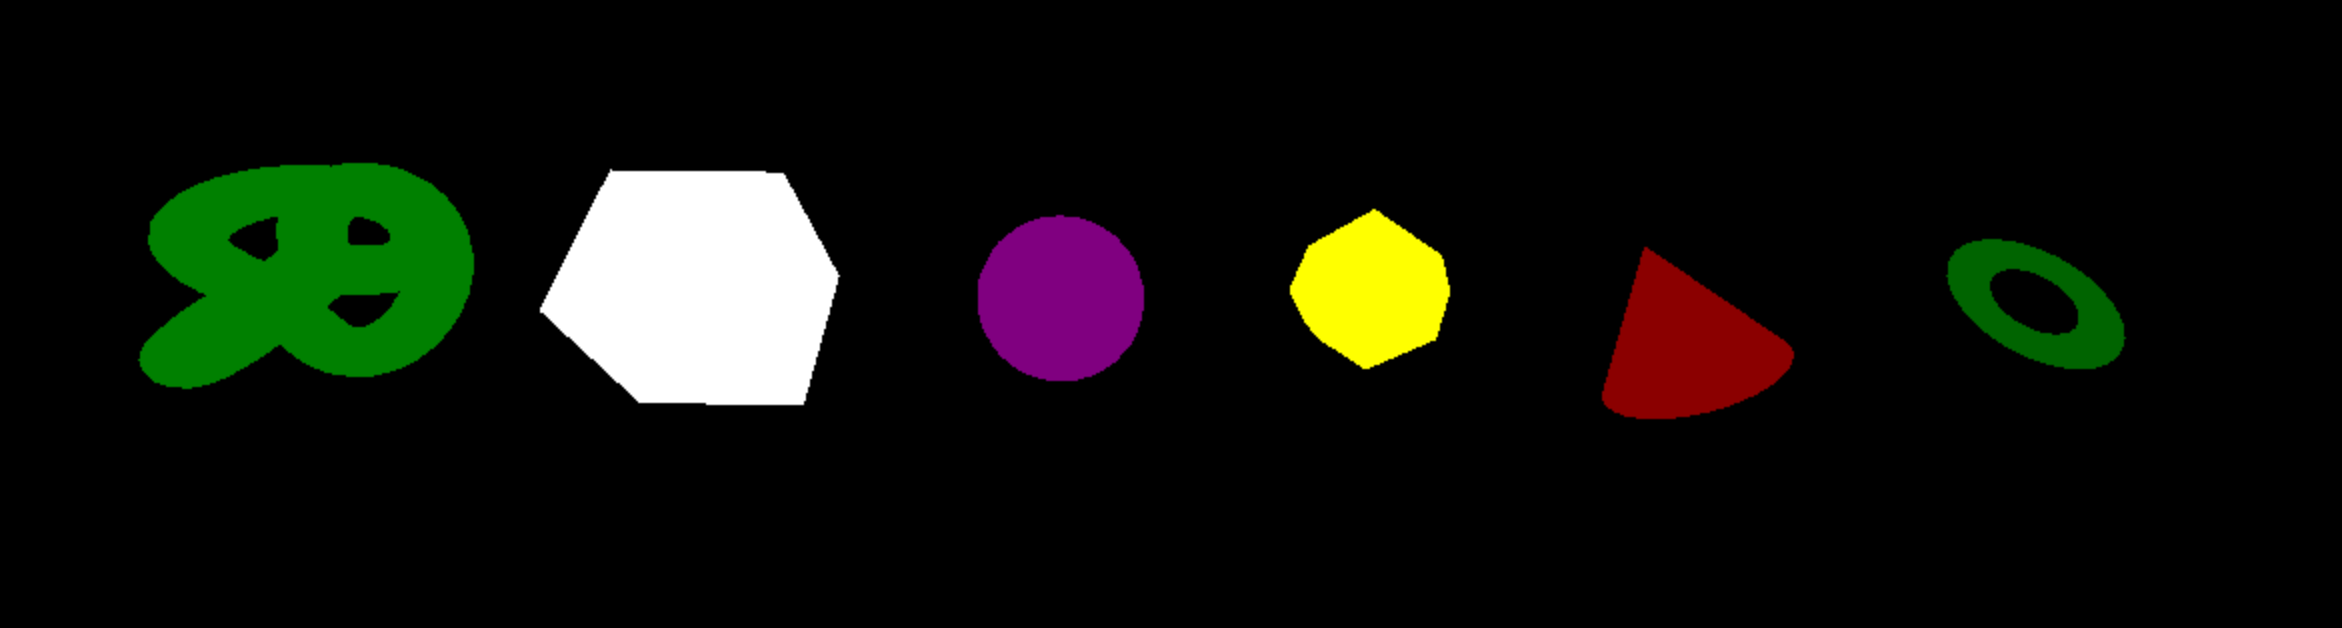
\includegraphics[width=.7\textwidth]{gfx/for-each-shapes.png}
\end{center}

\noindent\textbf{Please make sure that your code is accessible through Github Pages. Also, please commit this PDF and your final code to your Github fork, and submit a pull request.}

\vspace{.5cm} % add some space

Link to your assignment: \url{https://hltdev8642.github.io/cs460student/03/index.html}

\clearpage %%% new page for bonus questions

\noindent\textbf{Bonus (33 points):}


\vspace{.5cm} % add some space

\noindent Part 1 (5 points): Do you observe Z-Fighting? If yes, when?

\\~\\
Yes.
It is seen most at the points in the scene that have the highest density of geometries, or regions in which there are many overlapping objects/polygons.
\vspace{1cm}


\begin{center}
    
\includegraphics[width=1.0\textwidth]{gfx/z-fighting-investigation-image-1.png}
\end{center}

\vspace{3cm}

\clearpage

\noindent Part 2 (10 points): Please change \url{window.onclick} to \url{window.onmousemove}. Now, holding \url{SHIFT} and moving the mouse draws a ton of shapes. Submit your changed code as part of your \url{03/index.html} file and \textbf{please replace the screenshot below with your drawing}.

\begin{center}
    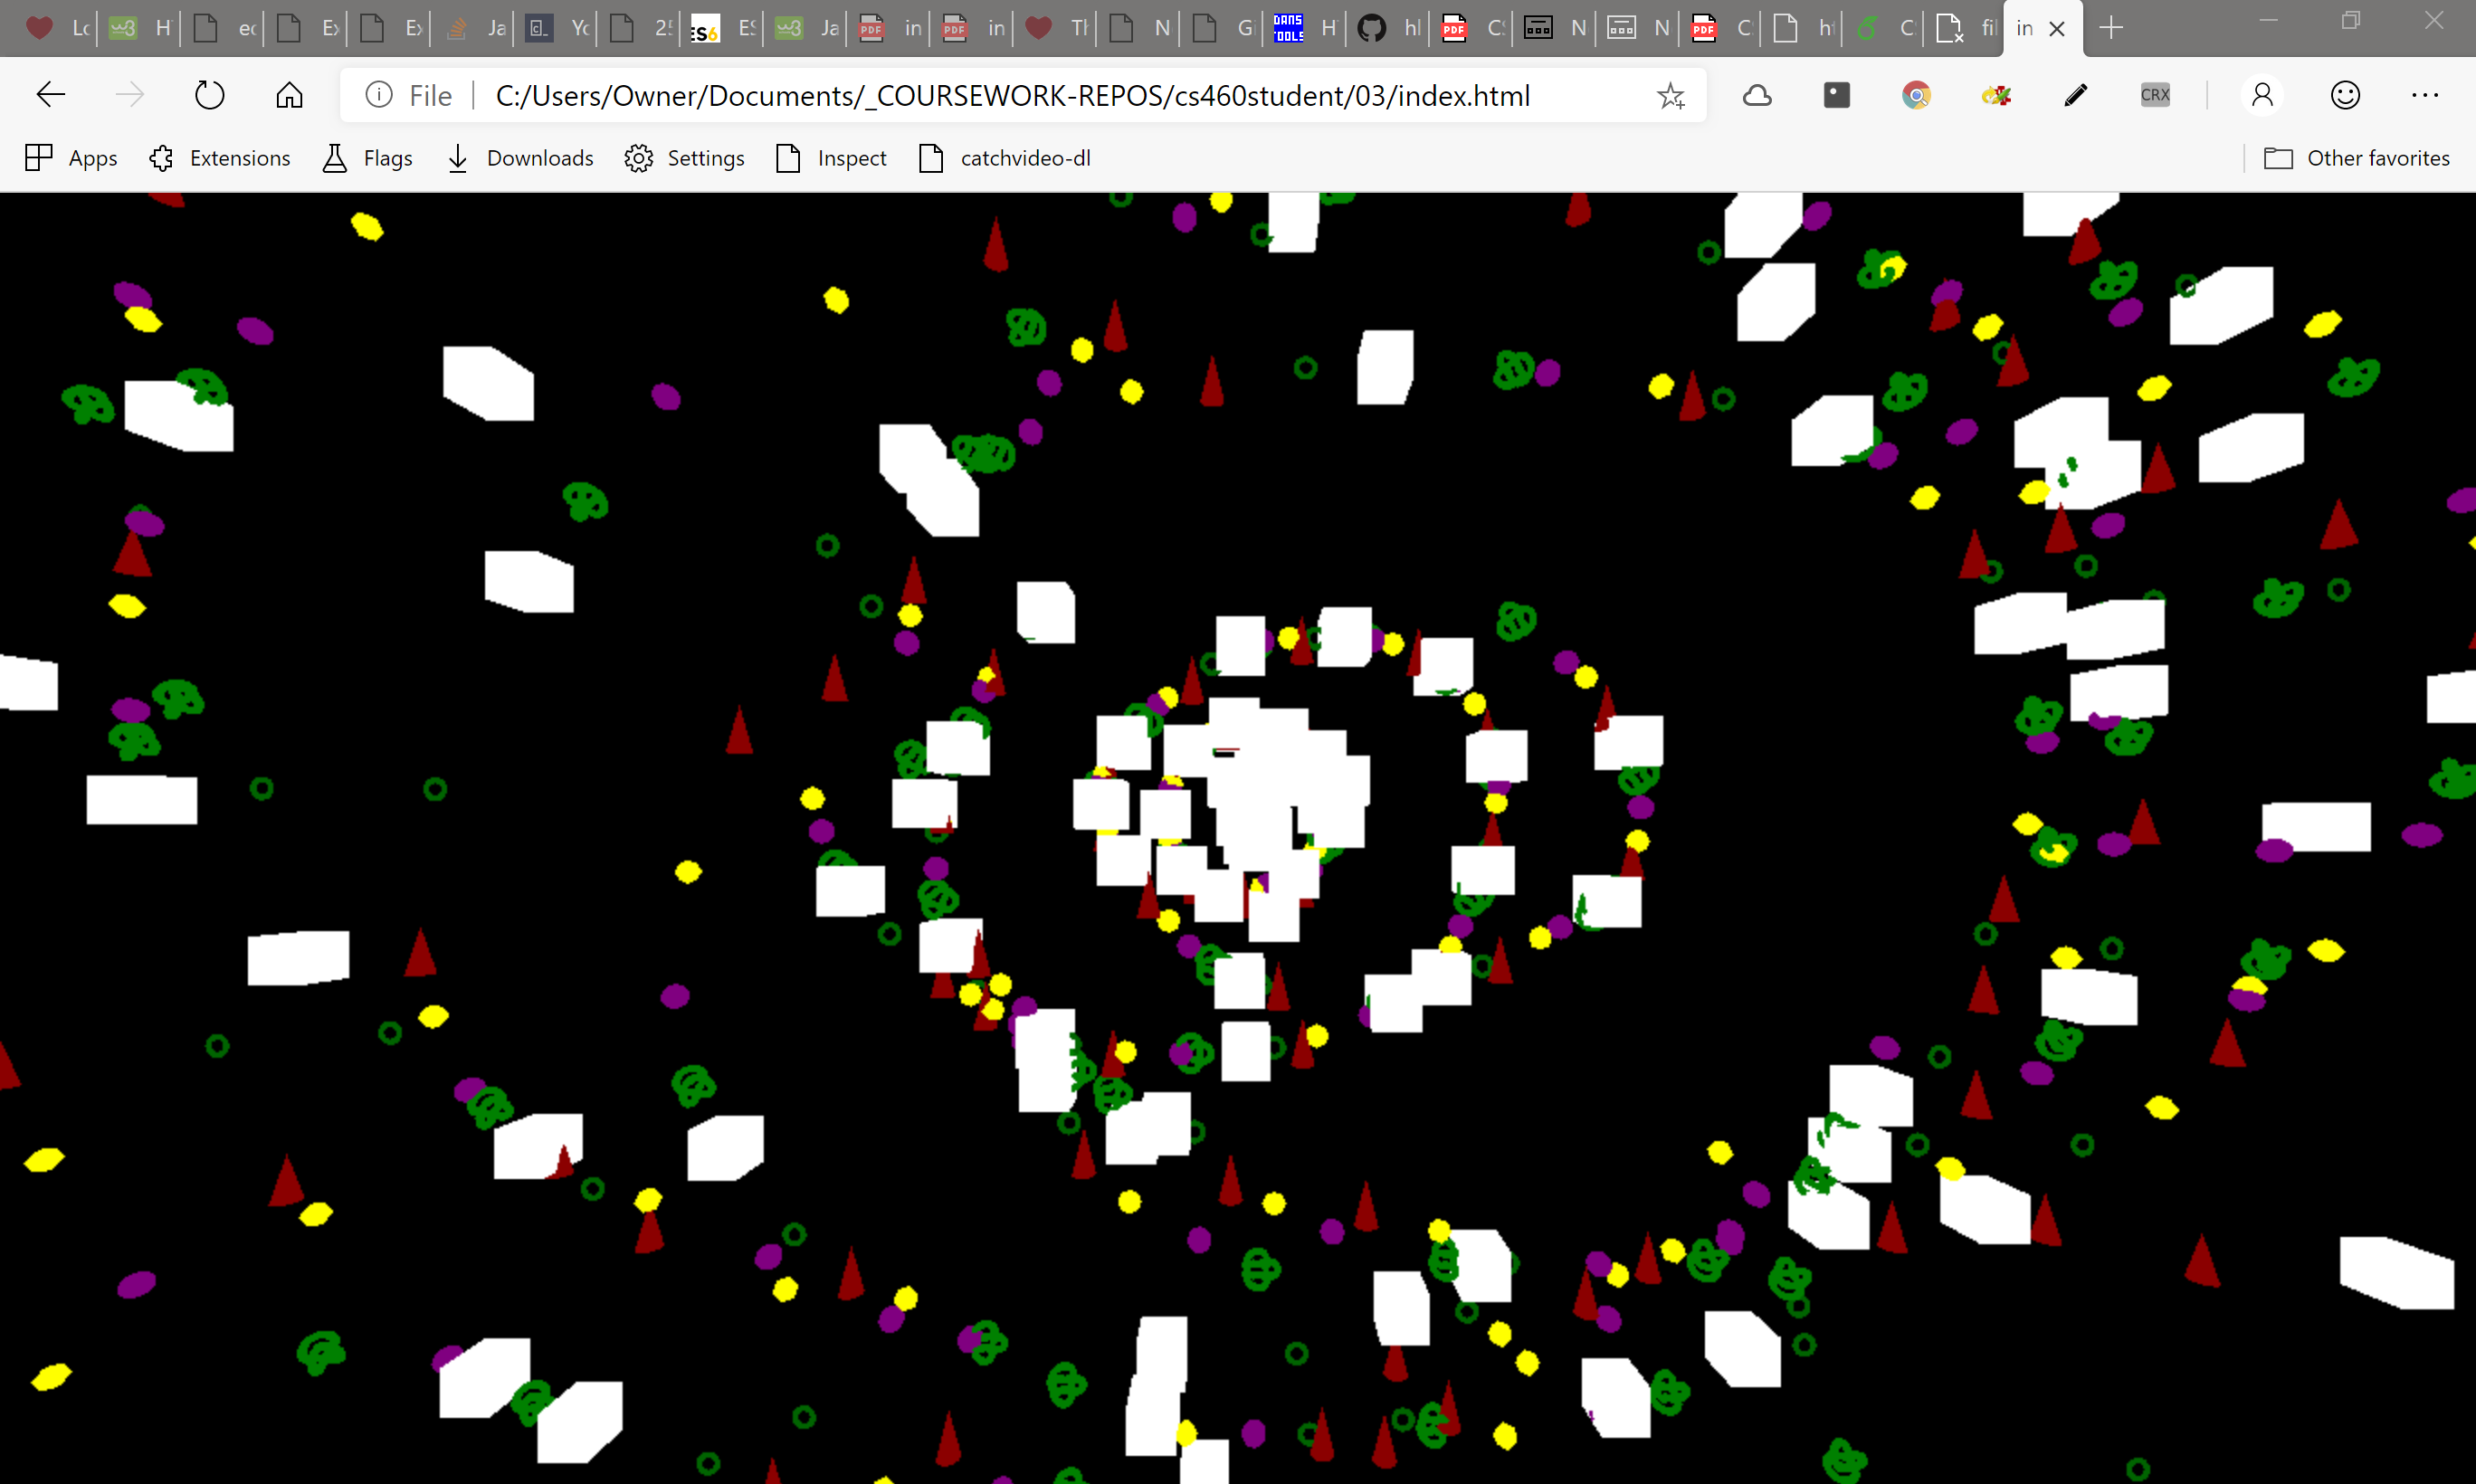
\includegraphics[width=.5\textwidth]{gfx/shape-galaxy-screenshot-1.png}
    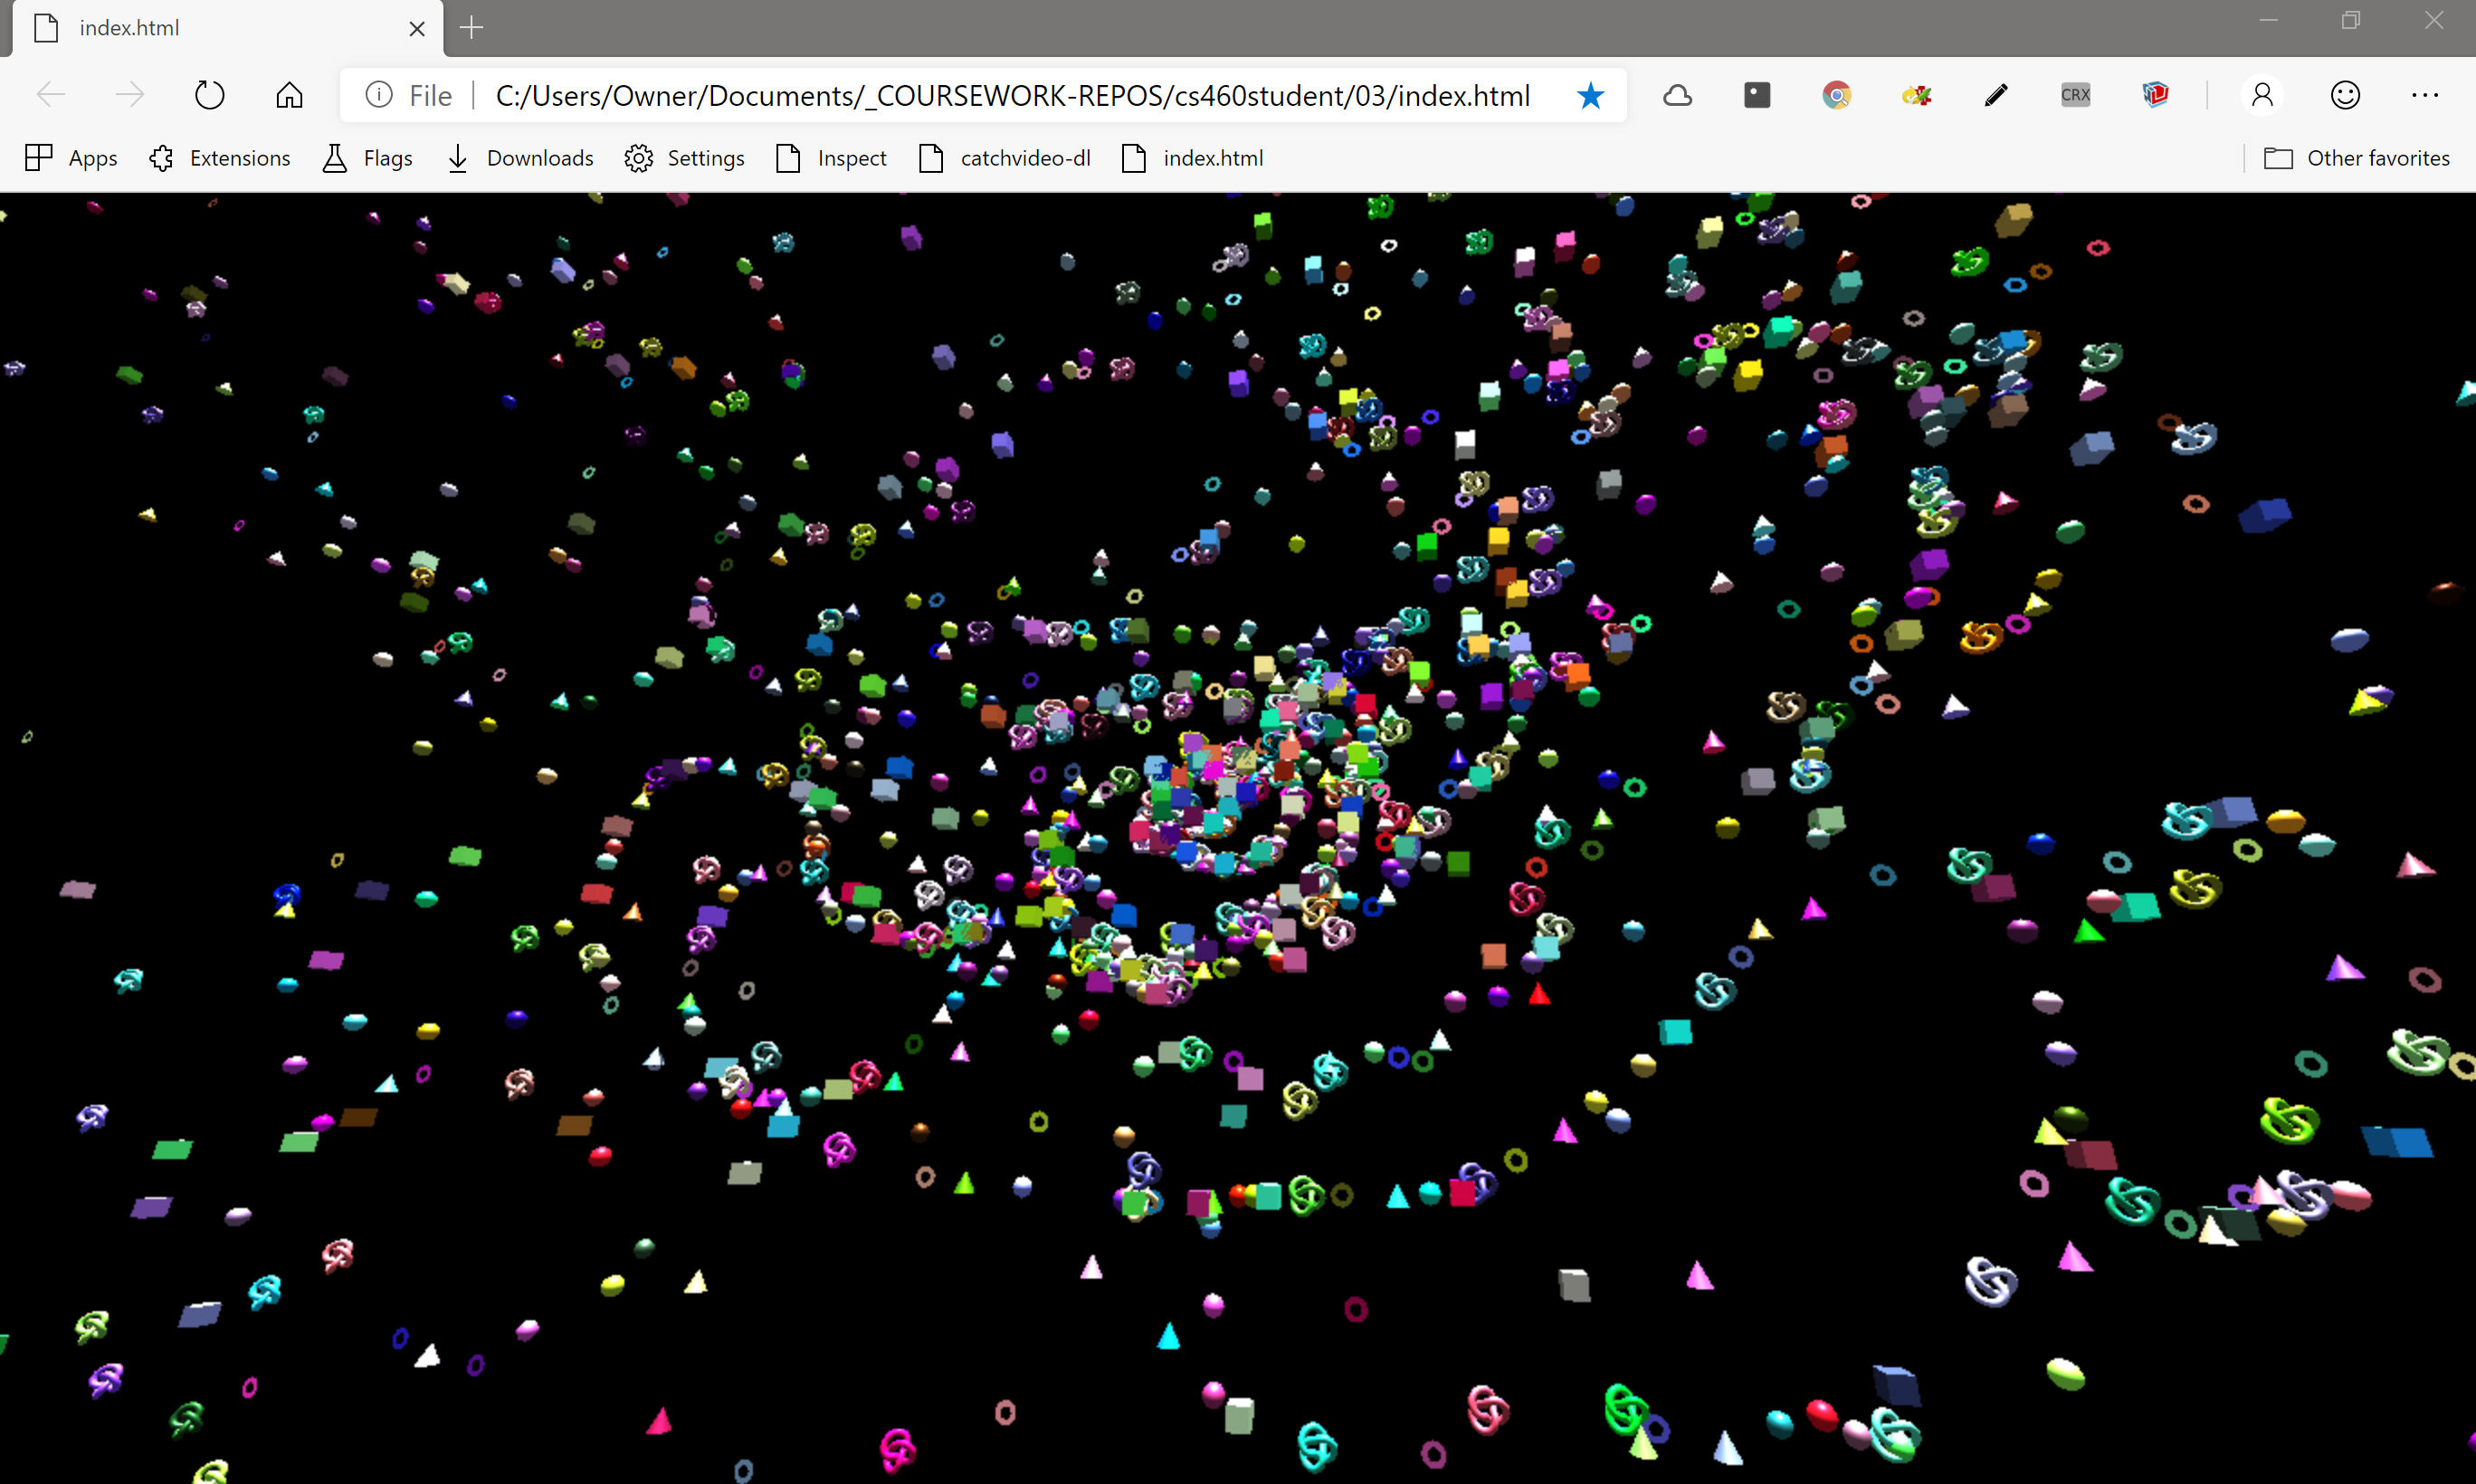
\includegraphics[width=.5\textwidth]{gfx/shape-galaxy-screenshot-2.png}
    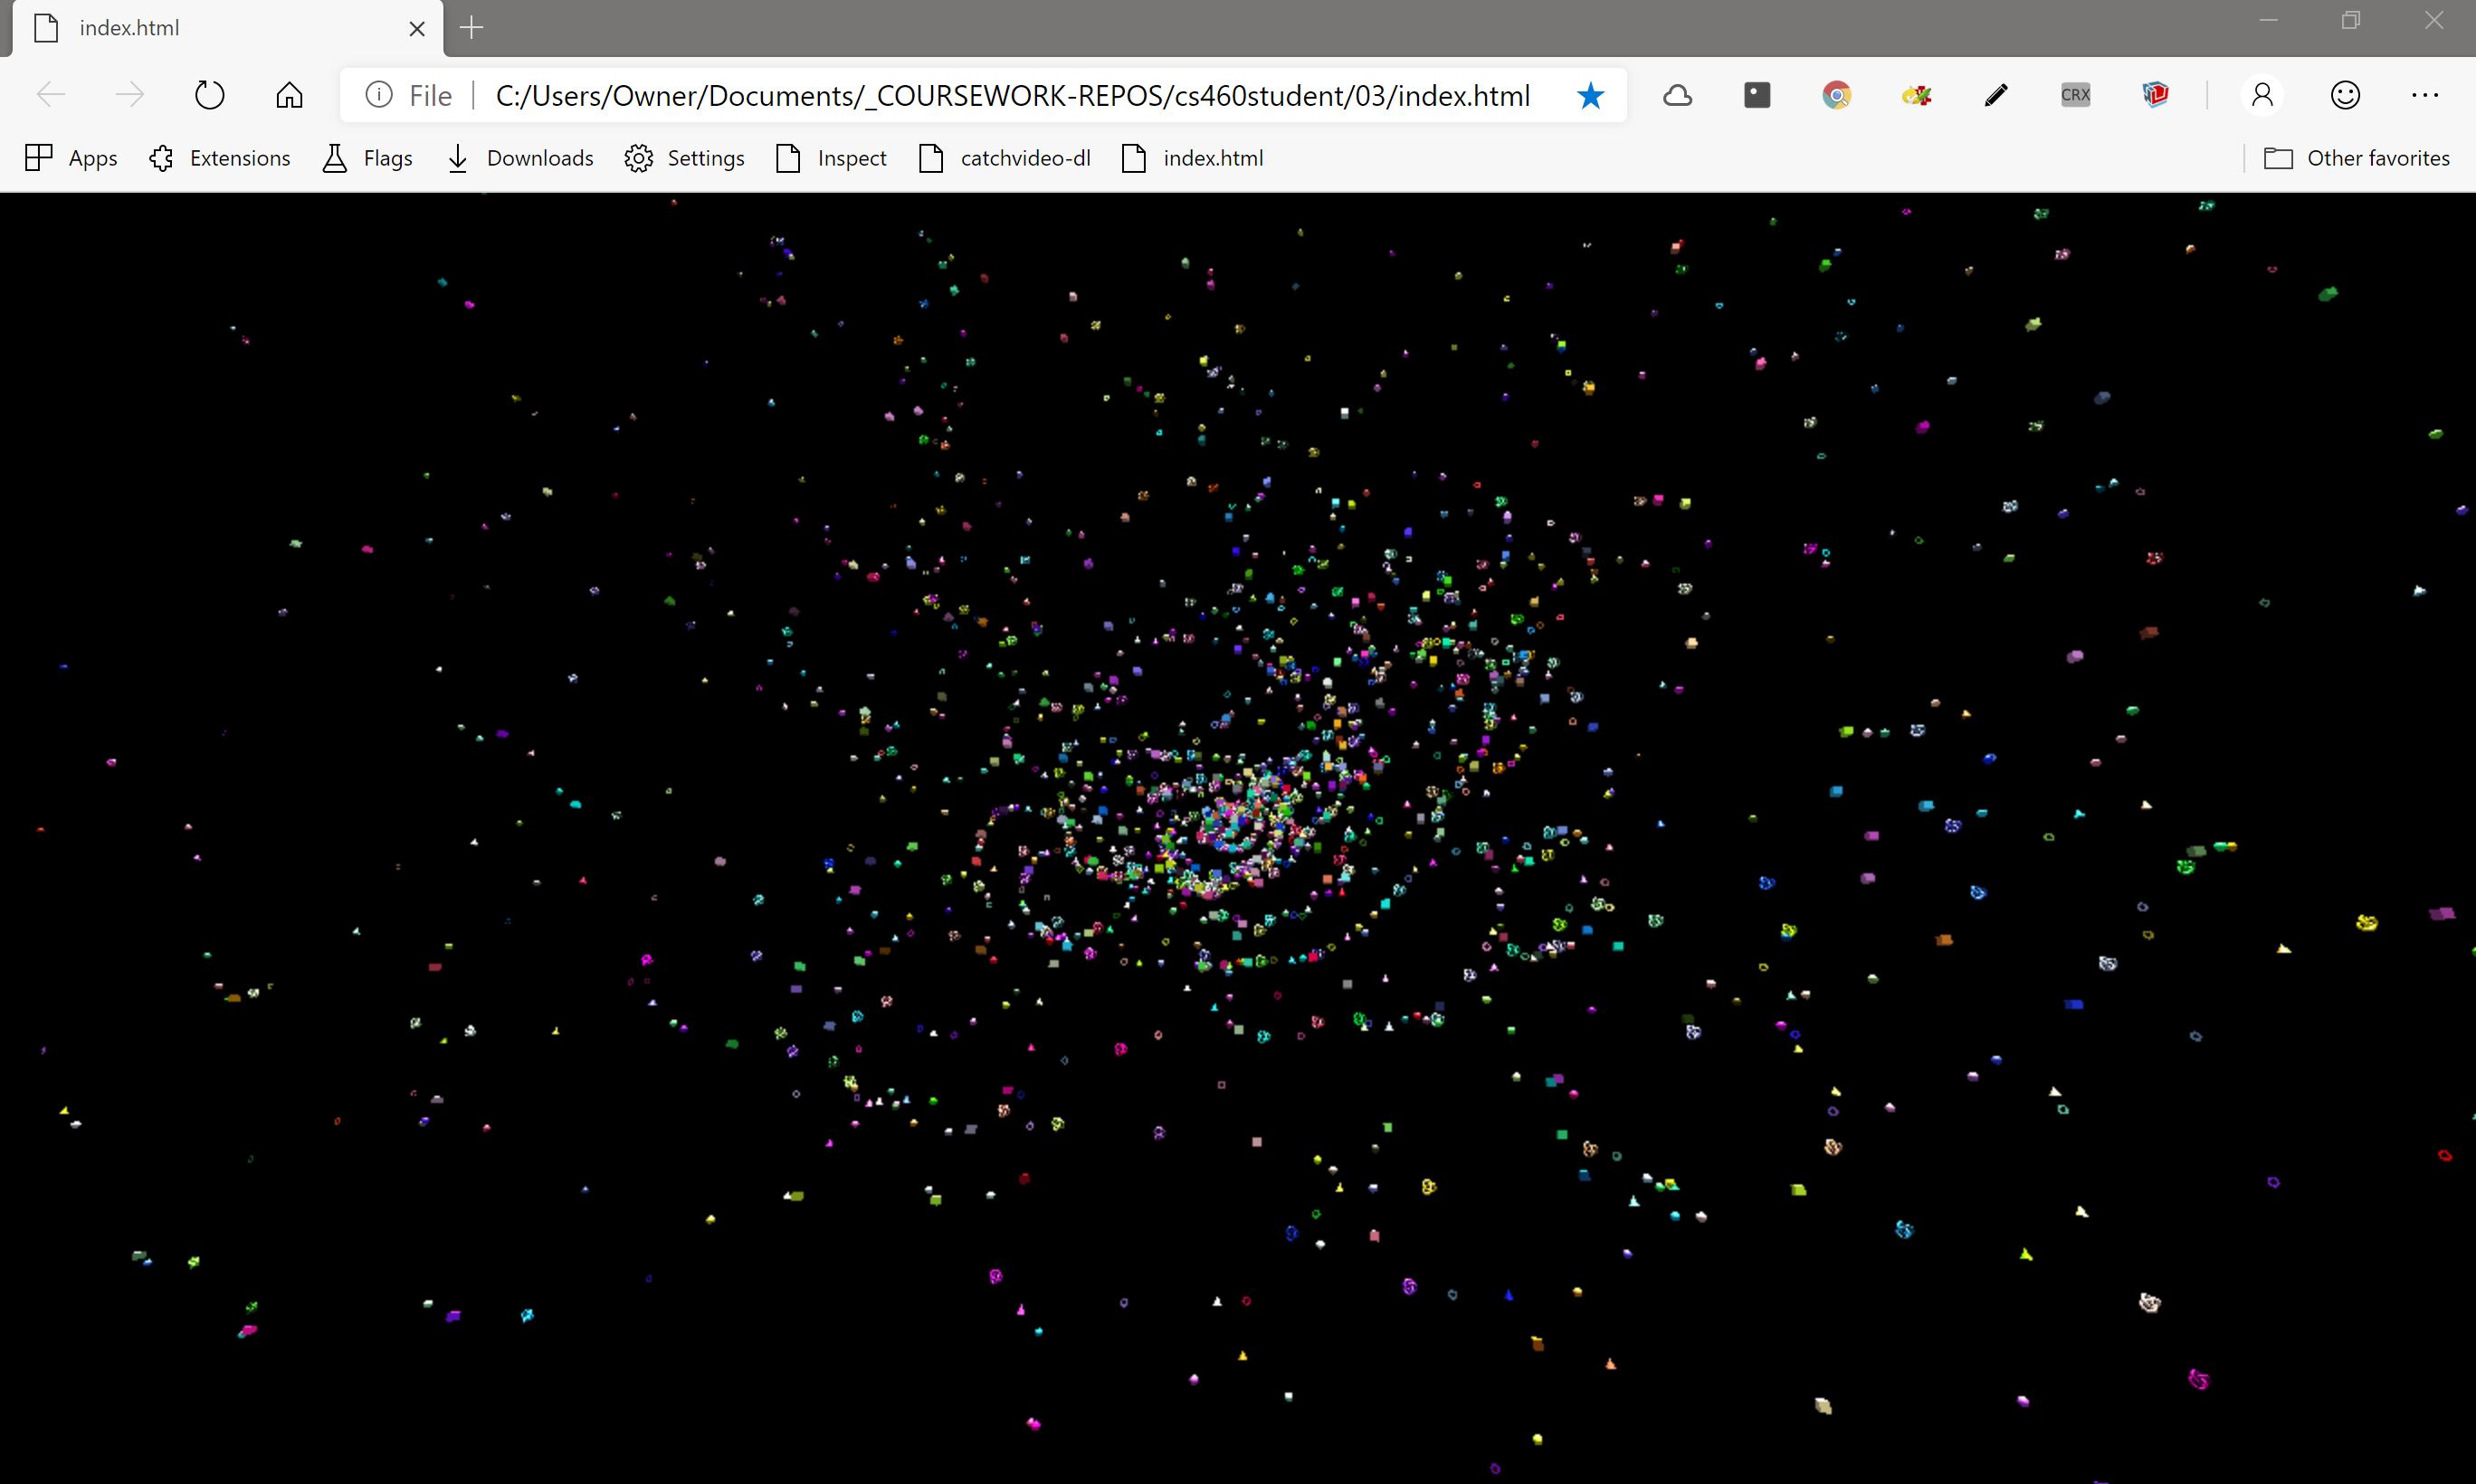
\includegraphics[width=.5\textwidth]{gfx/shape-galaxy-screenshot-3.png}
    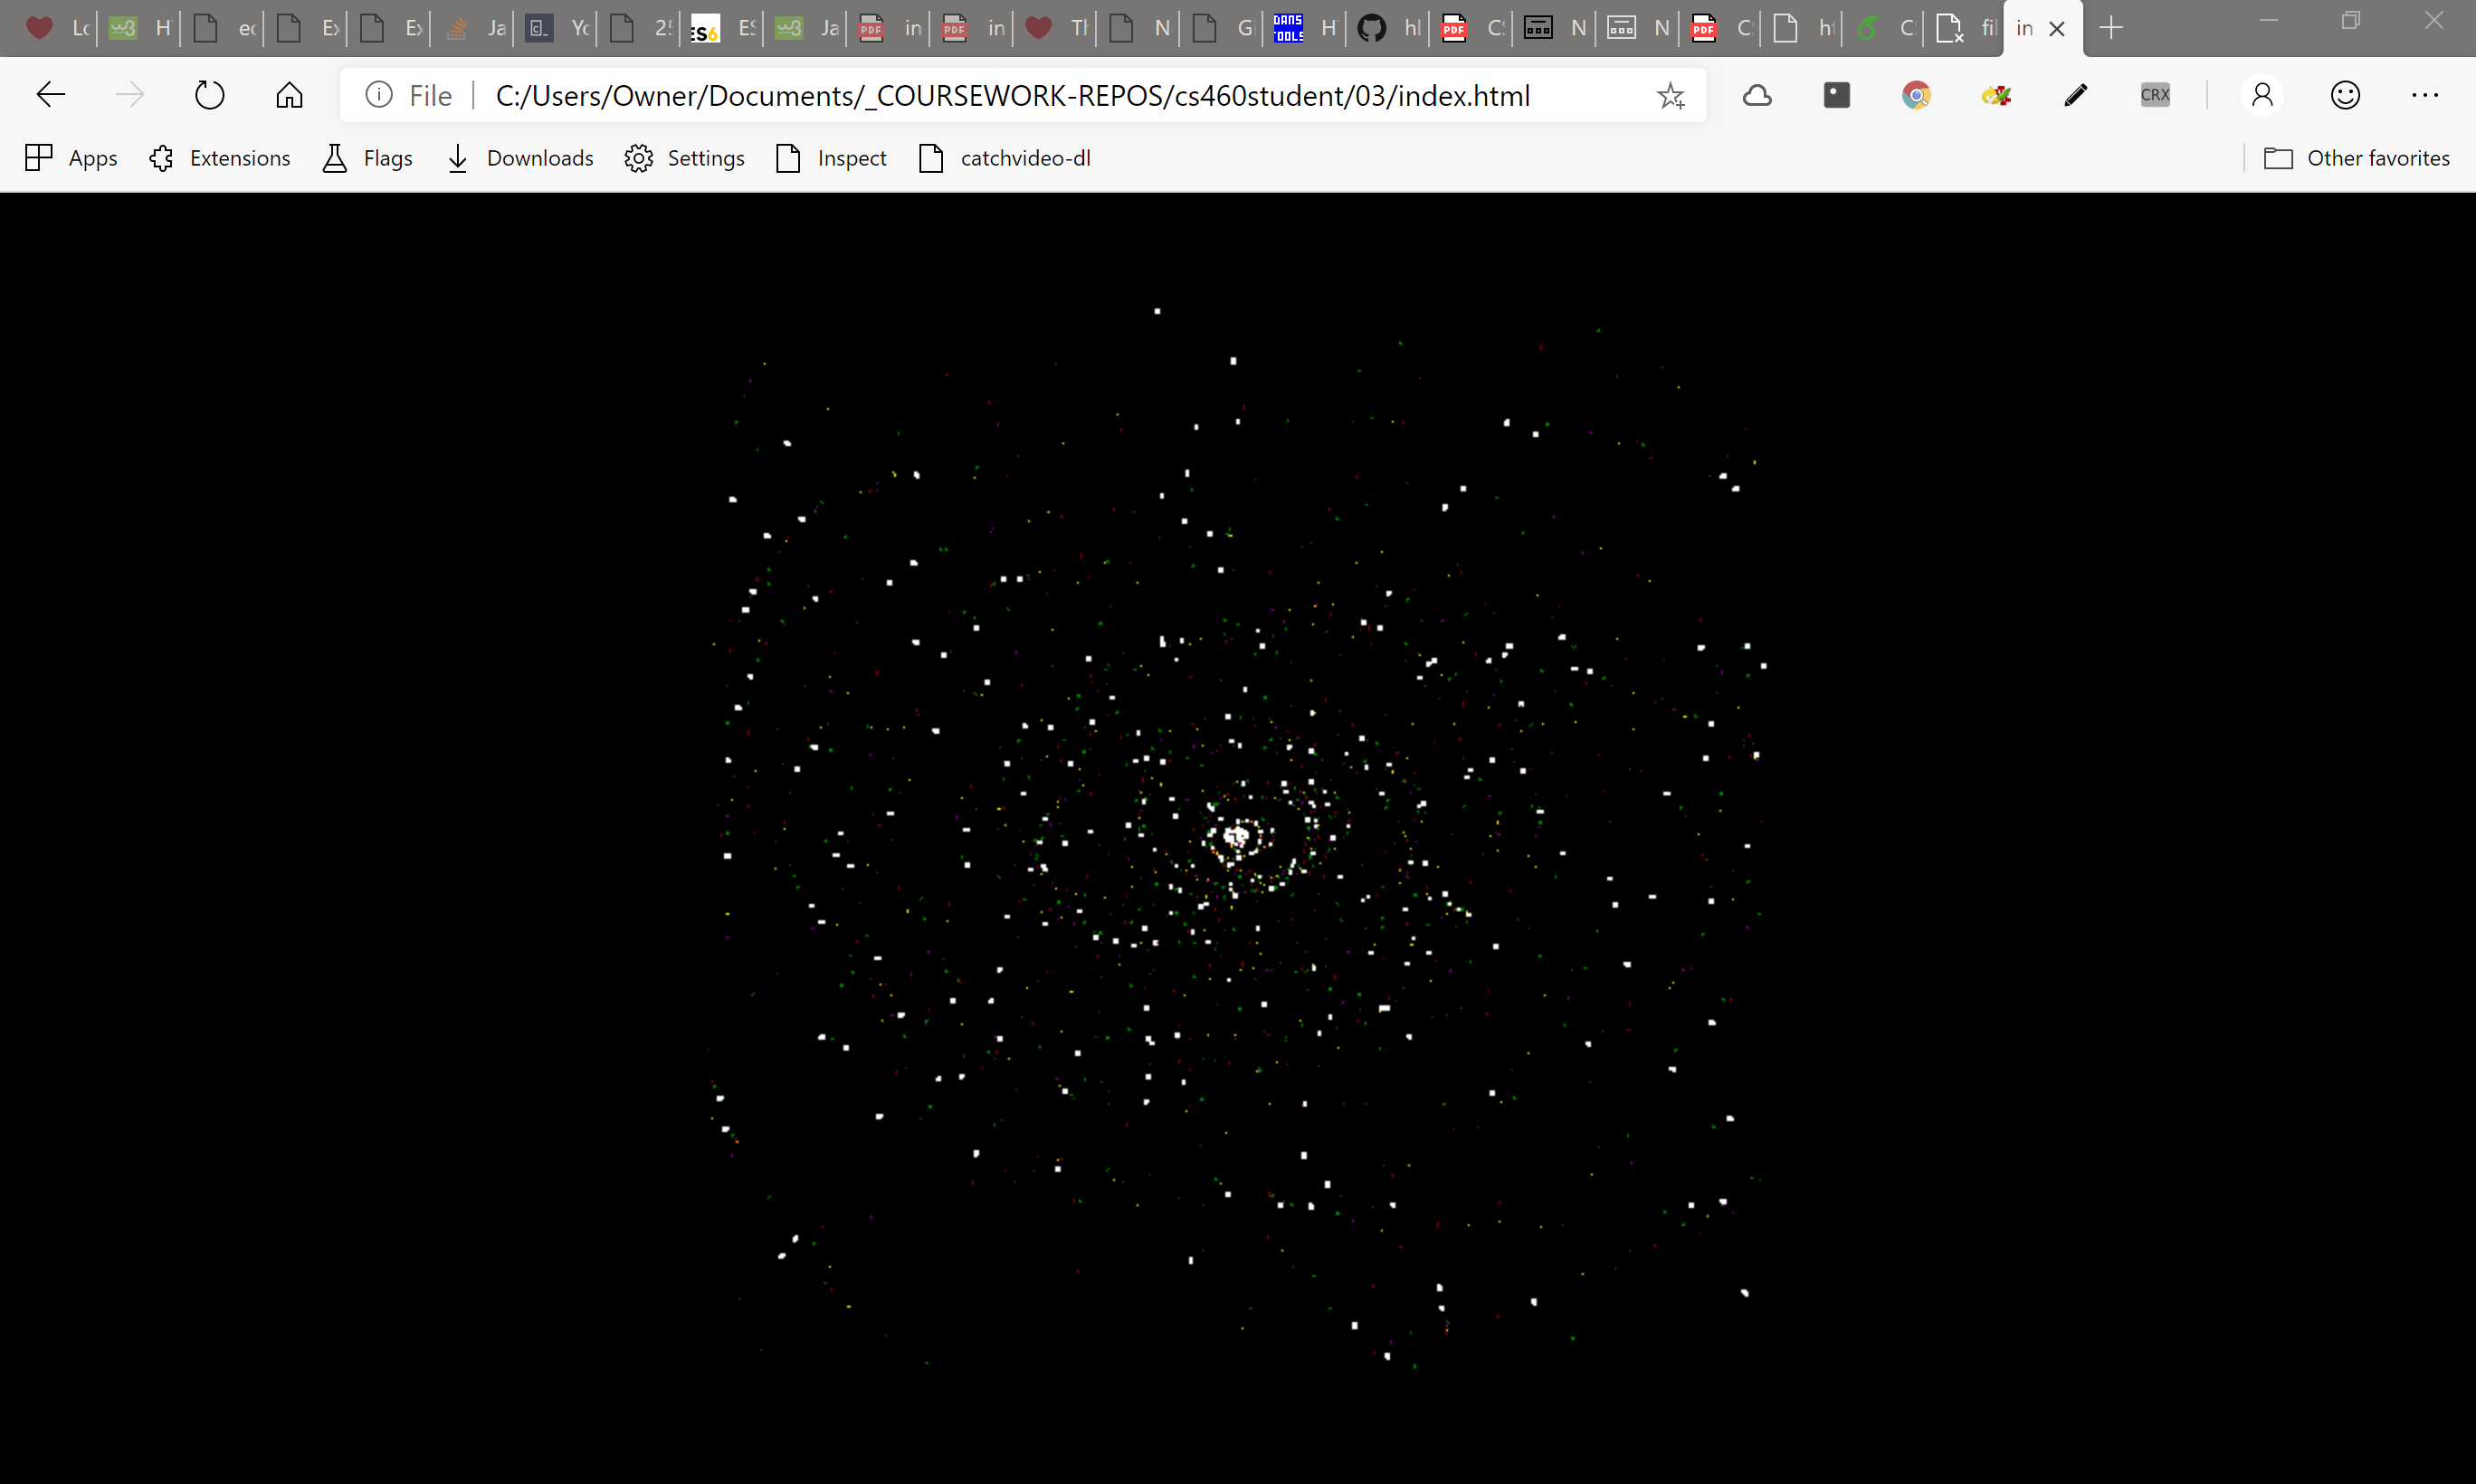
\includegraphics[width=.5\textwidth]{gfx/shape-galaxy-screenshot-4.png}
\end{center}

\vspace{2cm} % add some space

\noindent Part 3 (18 points): Please keep track of the number of placed objects and print the count in the JavaScript console. Now, with the change to \url{window.onmousemove}, after how many objects do you see a slower rendering performance? 
\\~\\
\noindent I honestly couldn't reach a number that it started to decline. The count I was at however was at 3441 objects and there still was very little noticeable drop in performance.

\vspace{.5cm}

\noindent However I realized through use of the Application/Memory inspector in chrome that my visual assessment of performance was probably not too accurate, as the trace revealed a very well-defined point in the runtime when the performance decreased. 

\vspace{.5cm}
(***See screenshot below***)
\vspace{1cm}


\begin{center}
    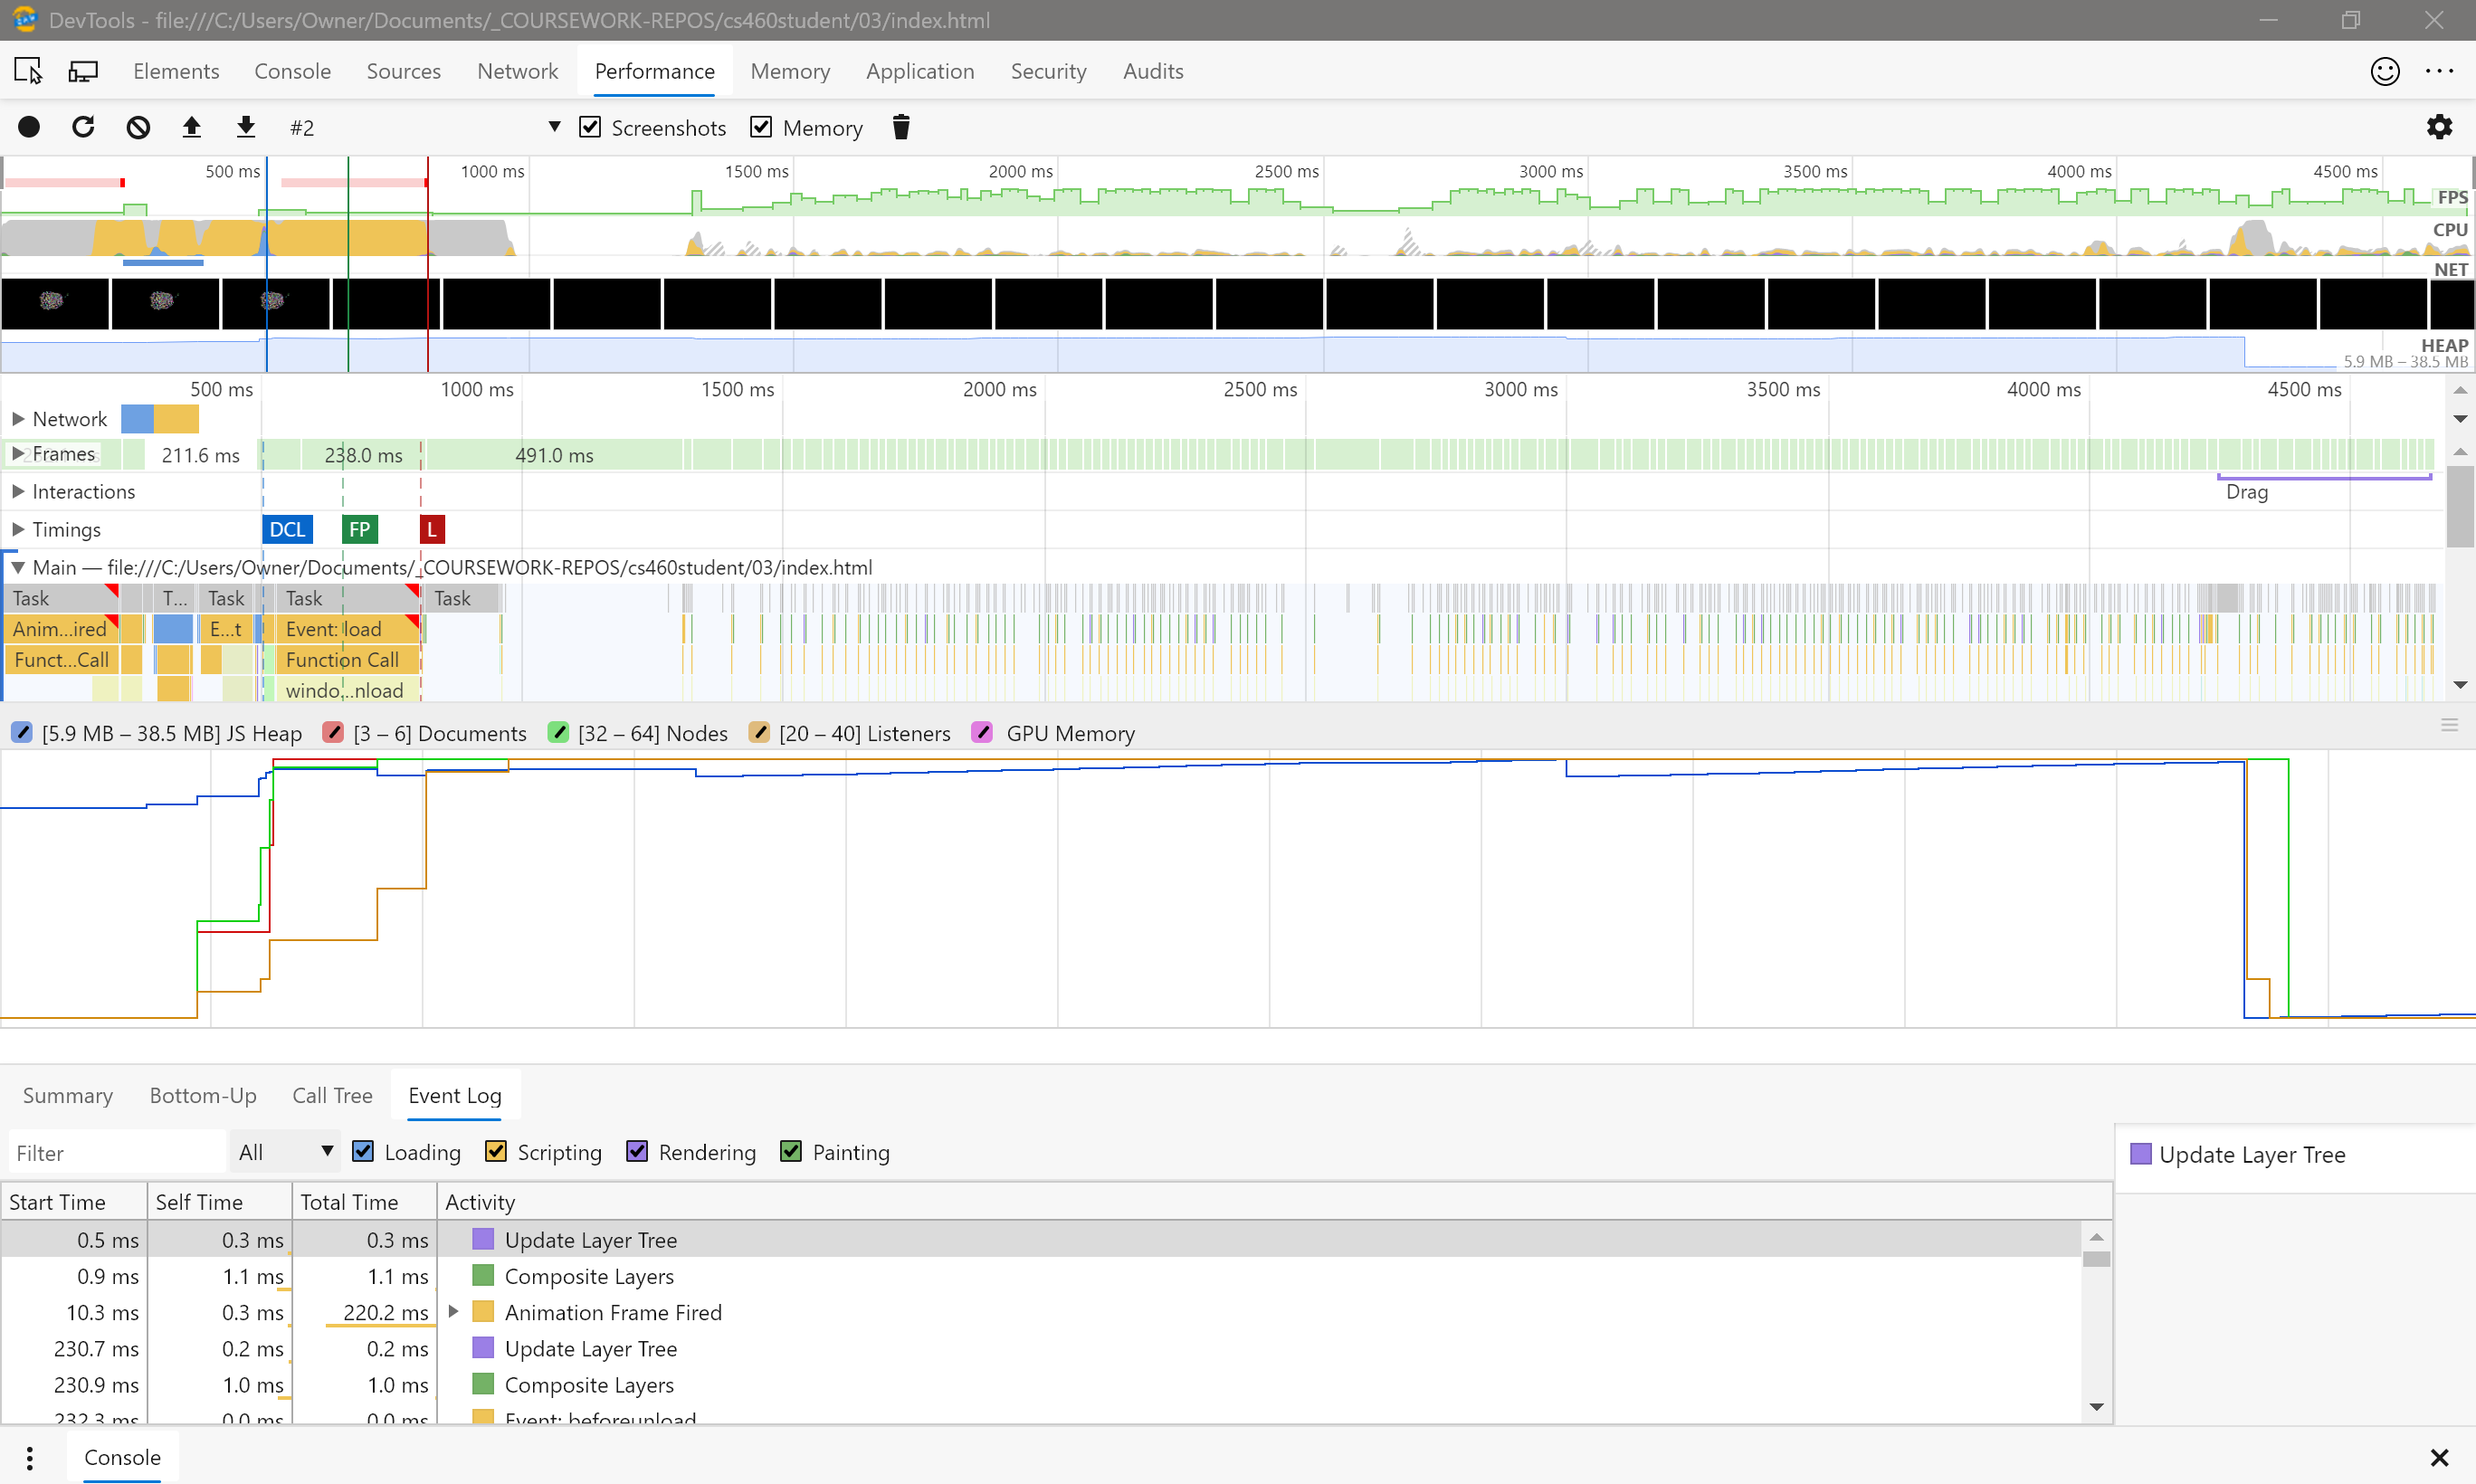
\includegraphics[width=1.0\textwidth]{gfx/performance-monitor-check-1.png}
\end{center}

\vspace{1cm}

\clearpage

\noindent What happens if the console is not open during drawing?
\\~\\
\noindent The performance \textit{may} have increased slightly, however it was nothing too significant if any. Also, it would be difficult to use the performance monitor (to check the performance), as this is ironically part of the console/inspector panel...
\vspace{1cm}

\noindent Can you estimate the total number of triangles drawn as soon as slow-down occurs?
\\~\\
\noindent A lot....
\vspace{.5cm}

\noindent Using the console command "renderer.info.render.triangles", I was able to determine that for one of each type of geometry the total number of triangles is \textbf{4164}.

\vspace{.5cm}


\noindent If we assume the slowdown happened at 3241 objects (as mentioned prior), that would be:
\noindent\textbf{4164 triangles per iteration X 3241 / 6 objects per iteration = (3241/6) * 4164}
\vspace{.5cm}

\noindent\underline{= A GRAND TOTAL OF (APPROX):} \textbf{1750140 triangles}

\end{document}
